\begin{tikzfigure}[CAD view of the ID31 end station]
\label{fig:assemblage}
\centering
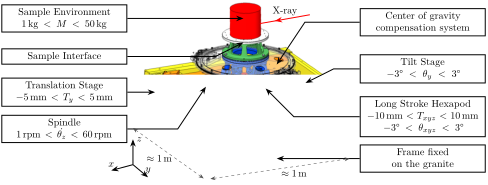
\includegraphics[width=\linewidth]{./figs/assemblage.pdf}


\end{tikzfigure}

\begin{minipage}[t]{0.49\linewidth}
  The ID31 Sample Station consists of multiple stacked stages
  (figs~\ref{fig:assemblage} and~\ref{fig:exp_setup}):



  \begin{itemize}
  \item \emph{translation stage}: travel range of \(T_y =
    \SI{\pm5}{\milli\metre}\). Permits to scan the sample through the X-ray.
  \item \emph{tilt stage}: rotates the sample around the \(y\) axis by
    \(\theta_y = \ang{\pm3}\). The rotation axis is aligned with the focusing
    point of the X-ray in order to allow experiments such as X-ray reflectivity.
  \item \emph{air bearing spindle}: rotate the sample around the vertical axis
    with an angular speed that varies from \(\dot{\theta_z} = \SI{1}{rpm}\) for
    light samples (\(M<\SI{1}{\kilo\gram}\)) to \(\dot{\theta_z} = \SI{60}{rpm}\)
    for heavy samples (\(M=\SI{50}{\kilo\gram}\)).
  \item \emph{long-stroke Stewart platform}: allows a fine positioning of the
    sample in all 6 degrees of freedom (DoF).
  \item \emph{gravity compensation system}: consists of two motorized mass that
    can be positioned around a circular guidance in order to perfectly aligned the
    center of mass with the spindle rotation axis.
  \item \emph{sample environment}: permits to study samples under wide range of
    condition: low (\(\SI{1.2}{\kelvin}\)) to high (\(\SI{2000}{\kelvin}\)) temperatures, high
    magnetic field (\(\SI{8}{\tesla}\)), etc.
  \end{itemize}
\end{minipage}\hfill
\begin{minipage}[t]{0.49\linewidth}
  \begin{tikzfigure}[Picture of the ID31 end station. (1) Granite, (2) Translation stage, (3) Tilt stage, (4) Long stroke hexapod, (5) Mass representing the sample environment. The spindle is hidden by the translation and tilt stages.]
  \label{fig:exp_setup}
  \centering
  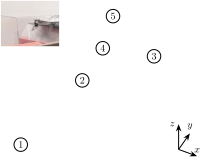
\includegraphics[width=\linewidth]{./figs/exp_setup.pdf}


  \end{tikzfigure}

  \begin{tikztable}[Specifications on the motions of the ID31 end station]
    \label{table:specifications}
    \centering
    \begin{tabular}{ccccc}
      \toprule
      & \(T_{xy}\) & \(T_z\) & \(\theta_y\) & \(\theta_z\)\\
      \midrule
      Repeatability & \(\SI{20}{\nano\metre}\) & \(\SI{10}{\nano\metre}\) & \(\SI{5}{\micro\radian}\) & \(\SI{2}{\micro\radian}\)\\
      MIM & \(\SI{3}{\nano\metre}\) & \(\SI{3}{\nano\metre}\) & \(\SI{2}{\micro\radian}\) & \(\SI{0.5}{\micro\radian}\)\\
      \bottomrule
    \end{tabular}
  \end{tikztable}
\end{minipage}\\

%%% Local Variables: ***
%%% mode:latex ***
%%% TeX-master: "2018 - Student Day.tex"  ***
%%% End: ***